\documentclass[10pt,mathserif]{beamer}

\usepackage{graphicx,amsmath,amssymb,tikz,psfrag}
\usepackage{pythonhighlight}

\input{preamble}

%% formatting

\mode<presentation>
{
\usetheme{default}
}
\setbeamertemplate{navigation symbols}{}
\usecolortheme[rgb={0.13,0.28,0.59}]{structure}
\setbeamertemplate{itemize subitem}{--}
\setbeamertemplate{frametitle} {
	\begin{center}
	  {\large\bf \insertframetitle}
	\end{center}
}

\newcommand\footlineon{
  \setbeamertemplate{footline} {
    \begin{beamercolorbox}[ht=2.5ex,dp=1.125ex,leftskip=.8cm,rightskip=.6cm]{structure}
      \footnotesize \insertsection
      \hfill
      {\insertframenumber}
    \end{beamercolorbox}
    \vskip 0.45cm
  }
}
\footlineon

\AtBeginSection[] 
{ 
	\begin{frame}<beamer> 
		\frametitle{Outline} 
		\tableofcontents[currentsection,currentsubsection] 
	\end{frame} 
} 

%% begin presentation

\title{\large \bfseries Bayesian Deep Learning}

\author{Kris Sankaran\\[3ex] Mila}

\date{\today}

\begin{document}

\section{Introduction}
\label{sec:introduction}

\begin{frame}
  \frametitle{Learning Objectives}
 \item Trace historical development of Bayesian ML, from Variational Inference
   to Bayesian Deep Learning
 \item Add some more models and algorithm to personal catalog of examples
 \item Understand underlying math and code for example algorithms
\end{frame}

\begin{frame}
  \frametitle{Papers from 1990}
  \begin{itemize}
  \item Gelfand and Smith: Renaissance in Bayesian Inference
  \item LeCun et. al.: Early proof of representation learning through neural networks
  \item Common: Use computation to automate tediour, expert-labor intensive processes
  \item Tension: The ``two cultures''... prediction or inference?
  \end{itemize}
  \begin{figure}
    \subfigure{\includegraphics[width=5cm]{figure/lecun}}
    \subfigure{\includegraphics[width=5cm]{figure/gelfand}}
  \end{figure}
\end{frame}

\begin{frame}
  \frametitle{Reconciliation}
  \begin{itemize}
  \item We need both inference and prediction for systems that \textit{sense}
    and \textit{act} in the real world
    \begin{itemize}
    \item Need systems running in real time, interfacing with the world
    \item Probabilistic descriptions give us much more to base our decisions off of
    \item It would be nice if everything were automatic, or at least modular
    \end{itemize}
  \item Bayesian deep learning: modular feature learning with uncertainty
  \end{itemize} 
  \begin{figure}
    \subfigure{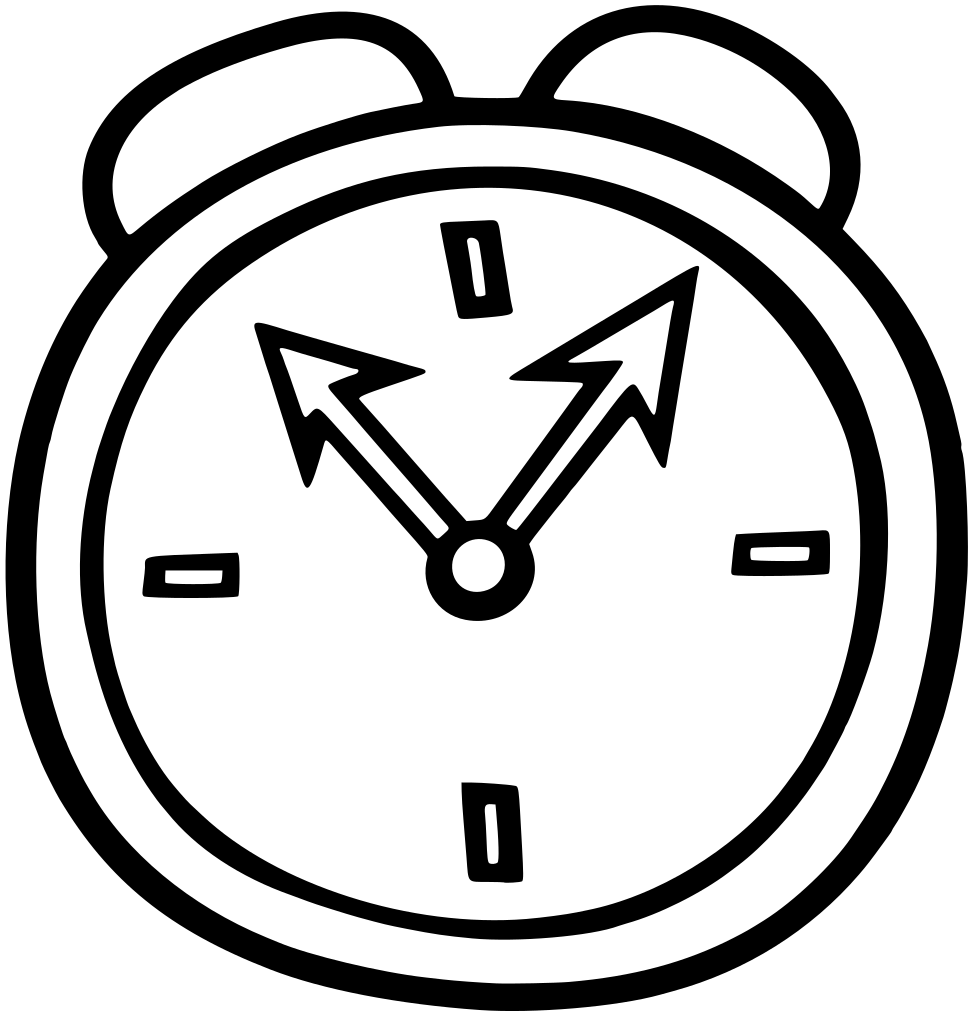
\includegraphics[width=3cm]{figure/clock}}
    \subfigure{\includegraphics[width=5cm]{figure/beeswarm}}
    \subfigure{\includegraphics[width=5cm]{figure/robot}}
  \end{figure}
\end{frame}

\begin{frame}
  \frametitle{Machine Learning checklist}
  Questions to ask every algorithm you meet.
 \begin{itemize}
 \item What is the model class?
 \item What is the evaluation criterion?
 \item What is the search strategy?
 \end{itemize} 
\end{frame}

\begin{frame}
  \frametitle{Machine Learning checklist}
  In a Bayesian context, should also ask,
  \begin{itemize}
  \item What is the generative mechanism? 
  \item What is the inference criterion?
  \item What is the algorithm?
  \end{itemize}
\end{frame}

\begin{frame}
  \frametitle{Classical Bayes}
  \begin{itemize}
  \item Bayes' Rule,
    \begin{align*}
      p\left(\theta \vert x\right) &= \frac{p\left(x \vert \theta\right)p\left(\theta\right)}{p\left(x\right)}
    \end{align*}
  \item Adapt your belief about $\theta$ after seeing $x$
  \item Specify likelihood $p\left(x \vert \theta\right)$ and prior $p\left(\theta\right)$
  \end{itemize} 
\end{frame}

\begin{frame}
  \frametitle{Example: Beta-Binomial}
  \begin{itemize}
  \item Task: Identify potential bias in a coin
  \item Model specification,
    \begin{itemize}
    \item Prior: $p \sim \Bet\left(a_0, b_0\right)$
    \item Likelihood: $x \vert p \sim \Bin\left(n, p\right)$
    \end{itemize}
  \item Posterior is still a beta
  \end{itemize} 
\begin{figure}[ht]
  \centering
  \includegraphics[width=0.6\paperwidth]{figure/betabinomial}
  \caption{\label{fig:betabinomial} }
\end{figure}
\end{frame}

\begin{frame}
  \frametitle{Beta-Binomial in Code}
  \begin{itemize}
  \item We can avoid doing any math by using the \texttt{pyro} package
  \item This is good practice for when it's impossible to do that math
  \item Hinges on the notion of a guide function
  \end{itemize} 
  \begin{python}
    # define the hyperparameters that control the beta prior
    alpha0 = torch.tensor(10.0)
    beta0 = torch.tensor(10.0)

    # sample f from the beta prior
    p = pyro.sample("heads_prob", dist.Beta(alpha0, beta0))
  \end{python}
  \begin{figure}[ht]
    \centering
    \includegraphics[options]{figure/pyro_model}
    \caption{\label{fig:pyro_model} }
  \end{figure}
\end{frame}

\begin{frame}
  \frametitle{Beta-Binomial in Code}
  \begin{itemize}
  \item We can avoid doing any math by using the \texttt{pyro} package
  \item This is good practice for when it's impossible to do that math
  \item Hinges on the notion of a guide function
  \end{itemize} 
  \begin{figure}[ht]
    \centering
    \includegraphics[options]{figure/pyro_inference}
    \caption{\label{fig:pyro_model} }
\end{figure}
\end{frame}

\section{Latent Variable Models}
\label{sec:latent_variable_models}

\begin{frame}
  \frametitle{Mixture Models}
  \begin{itemize}
  \item Sometimes, critical parts of data generating mechanisms are unobserved
    \item Need posterior inference over both mixture parameters $\mu_k,
      \Sigma_k$ as well as assignments $z_i$
  \end{itemize}  
  \begin{align*}
    \mu_{k} &\sim \Gsn\left(0, \Sigma_{0}\right) \\
    z_i &\sim \Cat\left(z_i \vert p\right) \\
    x_i \vert z_i = k &\sim \Gsn\left(x_i \vert \mu_{k}, \Sigma_k\right)
  \end{align*}
\end{frame}

\begin{frame}
  \frametitle{Other Examples}
  Many widely-used models depend on being able to work with latent variables,
  \begin{itemize}
  \item Exponential Family PCA
  \item Hidden Markov Models
  \item Latent Dirichlet Allocation
  \end{itemize} 
\end{frame}

\begin{frame}[]
  \frametitle{Mixture of Gaussians: Complete Data Likelihood}
  If we know the mixture assignments $z_i$ for each sample, we could write out
  the likelihood very explicitly.
  \begin{align*}
\log p\left(x, z\right) &= \log \left[\prod_{i = 1}^{n} \prod_{k = 1}^{K} \left(p_{k}\Gsn\left(x_i \vert \mu_k, \Sigma_k\right)^{\indic{z_i = k}}\right)\right] \\
&= \sum_{i = 1}^{n} \sum_{k = 1}^{K} \indic{z_i = k} \left[\log p_{k} + \log \Gsn\left(x_i \vert \mu_k, \Sigma_k\right)\right] \\
&= \sum_{i = 1}^{n} \sum_{k = 1}^{K} \indic{z_i = k} \left[\log p_{k} -\frac{D}{2}\log\left(2\pi\right) - \frac{1}{2}\log \left|\Sigma_k\right| -  \\ &\qquad\frac{1}{2} \left(x_i - \mu_k\right)^{T}\Sigma^{-1}_{k} \left(x_i - \mu_k)\right]
  \end{align*}
\end{frame}

\begin{frame}
  \frametitle{Marginalizing $z$}
  \begin{itemize}
  \item Can't use the previous derivation if we don't know the specific
    configuration of $z$
  \item Way too many configurations to actual do this sum
  \end{itemize} 
  \begin{align*}
    \log p\left(x\right) &= \log \sum_{z} p\left(x, z\right) dz
  \end{align*} 
\end{frame}

\begin{frame}
  \frametitle{Marginalizing $z$}
  \begin{itemize}
  \item This often makes posterior inference difficult too
  \item (There are workarounds for the Gaussian Mixture Model though)
  \end{itemize}
  \begin{align*}
    p\left(z \vert x\right) &= \frac{p\left(x \vert z\right)p\left(z\right)}{p\left(x\right)} \\
    &= \frac{p\left(x \vert z\right)p\left(z\right)}{\sum_{z} p\left(x, z\right)}
  \end{align*} 
\end{frame}

\begin{frame}
  \frametitle{Evidence Lower Bound}
  \begin{itemize}
  \item It's counterintuitive, but one problem-solving strategy is to deliberately introduce complexity
  \item Complexity $\rightarrow$ create additional degrees of freedom
  \end{itemize} 
\end{frame}

\begin{frame}
  \frametitle{Variational $q$}
  \begin{itemize}
  \item Consider some $q\left(z \vert x\right) \in \mathcal{Q}$, some large
    family of tractable densities
  \end{itemize} 
  \begin{align*}
    \log p\left(x\right) &= \Esubarg{q}{\log p\left(x\right)} \\
    &= \Esubarg{q}{\log \frac{p\left(x, z\right)}{p\left(z \vert x\right)}} \\
    &= \Esubarg{q}{\log \frac{p\left(x, z\right)}{q\left(z \vert x\right)} \frac{q\left(z \vert x\right)}{p\left(z \vert x\right)}} \\
    &= \Esubarg{q}{\log p\left(x \vert z\right)} - D_{KL}\left(q\left(z \vert x\right) \vert \vert p\left(z\right)\right) + D_{KL}\left(q\left(z \vert x\right) \vert \vert p\left(z \vert x\right)\right)
  \end{align*}
\end{frame}

\section{Variational Inference}
\label{sec:introduction}

\begin{frame}
  \frametitle{The Variational Idea}
  \begin{itemize}
  \item Transform integration problem into an optimization one
  \item Some families $\mathcal{Q}$ are easier to optimize over than others
  \end{itemize} 
\end{frame}


\section{Variational Autoencoders}

\end{document}
